\chapter{Result and Evaluation}
\label{ResultandEvaluation}

The simulations were done for both line and grid scenarios, as well as varying number of nodes and node distances (4, 9, 6 and 10m 50 100m respectively). Furthermore, for each topology both OF0 and MRHOF were simulated. A total of 100 separate simulations were performed for each scenario setup. The simulation results are arranged in four parts according to different simulation metrics, and each simulation metric is examined for individual scenario setup. 

\section{Packet Loss Rate}
\label{pl}

In the simulation a packet is considered to be lost when the echo packet is not received by the sender(in this case the root). 100 \texttt{UDPEcho} packets are sent from the root to each node in the network.

\subsection{Line scenario}
\label{pl:line}
Figure \ref{fig:pl_4_line_of0} and \ref{fig:pl_4_line_mrhof} show the mean packet loss rate for an OFO and MRHOF 4 nodes line scenario for inter-node distance of 10, 50 or 100 meters. Figure \ref{fig:pl_9_line_of0} to Figure \ref{fig:pl_16_line_mrhof} are the same except they show 6 and 9 nodes line scenarios.

\begin{figure}[htbp]
  \centering
    \leavevmode
    \subfloat[10 m]{\label{fig:4/OF0/line/dist10_montecarlo_contour_packetloss}
    \hspace{-25pt}
      \includegraphics[scale=0.23]{/home/bo/Documents/Thesis/Final/Template/Pics/results/4/OF0/line/dist10_montecarlo_contour_packetloss.pdf}}
     \subfloat[50 m]{\label{fig:4/OF0/line/dist50_montecarlo_contour_packetloss} 
     \hspace{-30pt}
      \includegraphics[scale=0.23]{/home/bo/Documents/Thesis/Final/Template/Pics/results/4/OF0/line/dist50_montecarlo_contour_packetloss.pdf}} 
     \subfloat[100 m]{\label{fig:4/OF0/line/dist100_montecarlo_contour_packetloss}
      \hspace{-30pt}
      \includegraphics[scale=0.23]{/home/bo/Documents/Thesis/Final/Template/Pics/results/4/OF0/line/dist100_montecarlo_contour_packetloss.pdf}}
  \caption{Mean Packet loss: 4 nodes line with OF0}
 \label{fig:pl_4_line_of0}
\end{figure}

\begin{figure}[htbp]
  \centering
    \leavevmode
    \subfloat[10 m]{\label{fig:4/MRHOF/line/dist10_montecarlo_contour_packetloss}
    \hspace{-25pt}
      \includegraphics[scale=0.23]{/home/bo/Documents/Thesis/Final/Template/Pics/results/4/MRHOF/line/dist10_montecarlo_contour_packetloss.pdf}}
     \subfloat[50 m]{\label{fig:4/MRHOF/line/dist50_montecarlo_contour_packetloss} 
     \hspace{-30pt}
      \includegraphics[scale=0.23]{/home/bo/Documents/Thesis/Final/Template/Pics/results/4/MRHOF/line/dist50_montecarlo_contour_packetloss.pdf}} 
     \subfloat[100 m]{\label{fig:4/MRHOF/line/dist100_montecarlo_contour_packetloss}
      \hspace{-30pt}
      \includegraphics[scale=0.23]{/home/bo/Documents/Thesis/Final/Template/Pics/results/4/MRHOF/line/dist100_montecarlo_contour_packetloss.pdf}}
  \caption{Mean Packet loss: 4 nodes line with MRHOF}
 \label{fig:pl_4_line_mrhof}
\end{figure}
      
\begin{figure}[htbp]
  \centering
    \leavevmode
    \subfloat[10 m]{\label{fig:9/OF0/line/dist10_montecarlo_contour_packetloss}
    \hspace{-25pt}
      \includegraphics[scale=0.23]{/home/bo/Documents/Thesis/Final/Template/Pics/results/9/OF0/line/dist10_montecarlo_contour_packetloss.pdf}}
     \subfloat[50 m]{\label{fig:9/OF0/line/dist50_montecarlo_contour_packetloss} 
     \hspace{-30pt}
      \includegraphics[scale=0.23]{/home/bo/Documents/Thesis/Final/Template/Pics/results/9/OF0/line/dist50_montecarlo_contour_packetloss.pdf}} 
     \subfloat[100 m]{\label{fig:4/OF0/line/dist100_montecarlo_contour_packetloss}
      \hspace{-30pt}
      \includegraphics[scale=0.23]{/home/bo/Documents/Thesis/Final/Template/Pics/results/9/OF0/line/dist100_montecarlo_contour_packetloss.pdf}}
  \caption{Mean Packet loss: 9 nodes line with OF0}
 \label{fig:pl_9_line_of0}
\end{figure}

\begin{figure}[htbp]
  %\centering
    \leavevmode
   % \hspace{-10pt}
    \subfloat[10 m]{\label{fig:9/MRHOF/line/dist10_montecarlo_contour_packetloss}
    \hspace{-25pt}
      \includegraphics[scale=0.23]{/home/bo/Documents/Thesis/Final/Template/Pics/results/9/MRHOF/line/dist10_montecarlo_contour_packetloss.pdf}}
     \subfloat[50 m]{\label{fig:9/MRHOF/line/dist50_montecarlo_contour_packetloss} 
     \hspace{-30pt}
      \includegraphics[scale=0.23]{/home/bo/Documents/Thesis/Final/Template/Pics/results/9/MRHOF/line/dist50_montecarlo_contour_packetloss.pdf}} 
     \subfloat[100 m]{\label{fig:9/MRHOF/line/dist100_montecarlo_contour_packetloss}
      \hspace{-30pt}
      \includegraphics[scale=0.23]{/home/bo/Documents/Thesis/Final/Template/Pics/results/9/MRHOF/line/dist100_montecarlo_contour_packetloss.pdf}}
  \caption{Mean Packet loss: 9 nodes line with MRHOF}
 \label{fig:pl_9_line_mrhof}
\end{figure}
   
\begin{figure}[htbp]
  \centering
    \leavevmode
    \subfloat[10 m]{\label{fig:16/OF0/line/dist10_montecarlo_contour_packetloss}
    \hspace{-25pt}
      \includegraphics[scale=0.23]{/home/bo/Documents/Thesis/Final/Template/Pics/results/16/OF0/line/dist10_montecarlo_contour_packetloss.pdf}}
     \subfloat[50 m]{\label{fig:16/OF0/line/dist50_montecarlo_contour_packetloss} 
     \hspace{-30pt}
      \includegraphics[scale=0.23]{/home/bo/Documents/Thesis/Final/Template/Pics/results/16/OF0/line/dist50_montecarlo_contour_packetloss.pdf}} 
     \subfloat[100 m]{\label{fig:16/OF0/line/dist100_montecarlo_contour_packetloss}
      \hspace{-30pt}
      \includegraphics[scale=0.23]{/home/bo/Documents/Thesis/Final/Template/Pics/results/16/OF0/line/dist100_montecarlo_contour_packetloss.pdf}}
  \caption{Mean Packet loss: 16 nodes line with OF0}
 \label{fig:pl_16_line_of0}
\end{figure}

\begin{figure}[htbp]
  \centering
    \leavevmode
    \subfloat[10 m]{\label{fig:16/MRHOF/line/dist10_montecarlo_contour_packetloss}
    \hspace{-25pt}
      \includegraphics[scale=0.23]{/home/bo/Documents/Thesis/Final/Template/Pics/results/16/MRHOF/line/dist10_montecarlo_contour_packetloss.pdf}}
     \subfloat[50 m]{\label{fig:16/MRHOF/line/dist50_montecarlo_contour_packetloss} 
     \hspace{-30pt}
      \includegraphics[scale=0.23]{/home/bo/Documents/Thesis/Final/Template/Pics/results/16/MRHOF/line/dist50_montecarlo_contour_packetloss.pdf}} 
     \subfloat[100 m]{\label{fig:16/MRHOF/line/dist100_montecarlo_contour_packetloss}
      \hspace{-30pt}
      \includegraphics[scale=0.23]{/home/bo/Documents/Thesis/Final/Template/Pics/results/16/MRHOF/line/dist100_montecarlo_contour_packetloss.pdf}}
  \caption{Mean Packet loss: 16 nodes line with MRHOF}
 \label{fig:pl_16_line_mrhof}
\end{figure}

For 4 nodes and 9 nodes line scenario, the packet loss performances under the same setup have no difference between OF0 and MRHOF. When the node number increases to 16, simulation with OF0 starts to exhibit a higher packet loss than MRHOF. In the 50 meters inter node distance case (Figure \ref{fig:16/OF0/line/dist50_montecarlo_contour_packetloss}), one can see a packet loss rate higher than 15\% in the last few nodes. This indicates the routes between the root and the nodes either broken, or have a low PRR. When the inter node distance increased to 100 meters, OF0 presents again a good case in terms of packet loss rate (Figure \ref{fig:16/OF0/line/dist100_montecarlo_contour_packetloss}). In the meanwhile, MRHOF continues to show a low packet loss rate.   
\newline 

\subsection{Grid Scenario}
\label{grid}
The same results for grid scenario are shown in Figure \ref{fig:pl_4_grid_of0} to Figure \ref{fig:pl_16_grid_mrhof}

\begin{figure}[htbp]
  \centering
    \leavevmode
    \subfloat[10 m]{\label{fig:4/OF0/grid/dist10_montecarlo_contour_packetloss}
    \hspace{-25pt}
      \includegraphics[scale=0.23]{/home/bo/Documents/Thesis/Final/Template/Pics/results/4/OF0/grid/dist10_montecarlo_contour_packetloss.pdf}}
     \subfloat[50 m]{\label{fig:4/OF0/grid/dist50_montecarlo_contour_packetloss} 
     \hspace{-30pt}
      \includegraphics[scale=0.23]{/home/bo/Documents/Thesis/Final/Template/Pics/results/4/OF0/grid/dist50_montecarlo_contour_packetloss.pdf}} 
     \subfloat[100 m]{\label{fig:4/OF0/grid/dist100_montecarlo_contour_packetloss}
      \hspace{-30pt}
      \includegraphics[scale=0.23]{/home/bo/Documents/Thesis/Final/Template/Pics/results/4/OF0/grid/dist100_montecarlo_contour_packetloss.pdf}}
  \caption{Mean Packet loss: 4 nodes grid with OF0}
 \label{fig:pl_4_grid_of0}
\end{figure}

\begin{figure}[htbp]
  \centering
    \leavevmode
    \subfloat[10 m]{\label{fig:4/MRHOF/grid/dist10_montecarlo_contour_packetloss}
    \hspace{-25pt}
      \includegraphics[scale=0.23]{/home/bo/Documents/Thesis/Final/Template/Pics/results/4/MRHOF/grid/dist10_montecarlo_contour_packetloss.pdf}}
     \subfloat[50 m]{\label{fig:4/MRHOF/grid/dist50_montecarlo_contour_packetloss} 
     \hspace{-30pt}
      \includegraphics[scale=0.23]{/home/bo/Documents/Thesis/Final/Template/Pics/results/4/MRHOF/grid/dist50_montecarlo_contour_packetloss.pdf}} 
     \subfloat[100 m]{\label{fig:4/MRHOF/grid/dist100_montecarlo_contour_packetloss}
      \hspace{-30pt}
      \includegraphics[scale=0.23]{/home/bo/Documents/Thesis/Final/Template/Pics/results/4/MRHOF/grid/dist100_montecarlo_contour_packetloss.pdf}}
  \caption{Mean Packet loss: 4 nodes grid with MRHOF}
 \label{fig:pl_4_grid_mrhof}
\end{figure}
      
\begin{figure}[htbp]
  \centering
    \leavevmode
    \subfloat[10 m]{\label{fig:9/OF0/grid/dist10_montecarlo_contour_packetloss}
    \hspace{-25pt}
      \includegraphics[scale=0.23]{/home/bo/Documents/Thesis/Final/Template/Pics/results/9/OF0/grid/dist10_montecarlo_contour_packetloss.pdf}}
     \subfloat[50 m]{\label{fig:9/OF0/grid/dist50_montecarlo_contour_packetloss} 
     \hspace{-30pt}
      \includegraphics[scale=0.23]{/home/bo/Documents/Thesis/Final/Template/Pics/results/9/OF0/grid/dist50_montecarlo_contour_packetloss.pdf}} 
     \subfloat[100 m]{\label{fig:4/OF0/grid/dist100_montecarlo_contour_packetloss}
      \hspace{-30pt}
      \includegraphics[scale=0.23]{/home/bo/Documents/Thesis/Final/Template/Pics/results/9/OF0/grid/dist100_montecarlo_contour_packetloss.pdf}}
  \caption{Mean Packet loss: 9 nodes grid with OF0}
 \label{fig:pl_9_grid_of0}
\end{figure}

\begin{figure}[htbp]
  %\centering
    \leavevmode
   % \hspace{-10pt}
    \subfloat[10 m]{\label{fig:9/MRHOF/grid/dist10_montecarlo_contour_packetloss}
    \hspace{-25pt}
      \includegraphics[scale=0.23]{/home/bo/Documents/Thesis/Final/Template/Pics/results/9/MRHOF/grid/dist10_montecarlo_contour_packetloss.pdf}}
     \subfloat[50 m]{\label{fig:9/MRHOF/grid/dist50_montecarlo_contour_packetloss} 
     \hspace{-30pt}
      \includegraphics[scale=0.23]{/home/bo/Documents/Thesis/Final/Template/Pics/results/9/MRHOF/grid/dist50_montecarlo_contour_packetloss.pdf}} 
     \subfloat[100 m]{\label{fig:9/MRHOF/grid/dist100_montecarlo_contour_packetloss}
      \hspace{-30pt}
      \includegraphics[scale=0.23]{/home/bo/Documents/Thesis/Final/Template/Pics/results/9/MRHOF/grid/dist100_montecarlo_contour_packetloss.pdf}}
  \caption{Mean Packet loss: 9 nodes grid with MRHOF}
 \label{fig:pl_9_grid_mrhof}
\end{figure}
   
\begin{figure}[htbp]
  \centering
    \leavevmode
    \subfloat[10 m]{\label{fig:16/OF0/grid/dist10_montecarlo_contour_packetloss}
    \hspace{-25pt}
      \includegraphics[scale=0.23]{/home/bo/Documents/Thesis/Final/Template/Pics/results/16/OF0/grid/dist10_montecarlo_contour_packetloss.pdf}}
     \subfloat[50 m]{\label{fig:16/OF0/grid/dist50_montecarlo_contour_packetloss} 
     \hspace{-30pt}
      \includegraphics[scale=0.23]{/home/bo/Documents/Thesis/Final/Template/Pics/results/16/OF0/grid/dist50_montecarlo_contour_packetloss.pdf}} 
     \subfloat[100 m]{\label{fig:4/OF0/grid/dist100_montecarlo_contour_packetloss}
      \hspace{-30pt}
      \includegraphics[scale=0.23]{/home/bo/Documents/Thesis/Final/Template/Pics/results/16/OF0/grid/dist100_montecarlo_contour_packetloss.pdf}}
  \caption{Mean Packet loss: 16 nodes grid with OF0}
 \label{fig:pl_16_grid_of0}
\end{figure}

\begin{figure}[htbp]
  \centering
    \leavevmode
    \subfloat[10 m]{\label{fig:16/MRHOF/grid/dist10_montecarlo_contour_packetloss}
    \hspace{-25pt}
      \includegraphics[scale=0.23]{/home/bo/Documents/Thesis/Final/Template/Pics/results/16/MRHOF/grid/dist10_montecarlo_contour_packetloss.pdf}}
     \subfloat[50 m]{\label{fig:16/MRHOF/grid/dist50_montecarlo_contour_packetloss} 
     \hspace{-30pt}
      \includegraphics[scale=0.23]{/home/bo/Documents/Thesis/Final/Template/Pics/results/16/MRHOF/grid/dist50_montecarlo_contour_packetloss.pdf}} 
     \subfloat[100 m]{\label{fig:16/MRHOF/grid/dist100_montecarlo_contour_packetloss}
      \hspace{-30pt}
      \includegraphics[scale=0.23]{/home/bo/Documents/Thesis/Final/Template/Pics/results/16/MRHOF/grid/dist100_montecarlo_contour_packetloss.pdf}}
  \caption{Mean Packet loss: 16 nodes grid with MRHOF}
 \label{fig:pl_16_grid_mrhof}
\end{figure}

Compared to line scenario, grid scenario is more complicated in the terms of routing due to its higher node density.  Under this scenario, OF0 shows a high packet loss in 16 nodes with 50 inter node distance (Figure \ref{fig:16/OF0/grid/dist50_montecarlo_contour_packetloss}) while MRHOF gives no more than 5\% packet loss. Furthermore, the packet loss rate of OF0 is also higher than that of MRHOF for 16 nodes with 100 meters inter node distance. 
\newline

The packet loss rate comparison between MRHOF and OF0 shows that with OF0 a node is very likely to choose a routing parent with a unreliable link, such as a link with a low PRR; on the other hand, MRHOF with link ETX is guaranteed to choose the link with the least estimated transmission count, therefore the parent choosing mechanism is more stable and reliable. 

\section{Route Trip Time}
\label{rtt}
 
\subsection{Line Scenario}
\label{line scenario}

The mean RTT for various node numbers and inter node distances of line scenario are shown in Figure \ref{fig:rtt_4_line_of0} to Figure \ref{fig:rtt_16_line_mrhof}.
\newline

Same as the mean packet loss rate results, the mean RTT performances of OF0 and MRHOF begin to divide in the 16 nodes topology. In Figure \ref{fig:16/OF0/line/dist50_montecarlo_contour} due to the bad routes between the root and a few further away nodes, the mean RTT becomes higher than 250 ms while MRHOF keeps a mean RTT within 150 ms even for the furthest node.
    
\begin{figure}[htbp]
  \centering
    \leavevmode
    \subfloat[10 m]{\label{fig:4/OF0/line/dist10_montecarlo_contour}
    \hspace{-25pt}
      \includegraphics[scale=0.23]{/home/bo/Documents/Thesis/Final/Template/Pics/results/4/OF0/line/dist10_montecarlo_contour.pdf}}
     \subfloat[50 m]{\label{fig:4/OF0/line/dist50_montecarlo_contour} 
     \hspace{-30pt}
      \includegraphics[scale=0.23]{/home/bo/Documents/Thesis/Final/Template/Pics/results/4/OF0/line/dist50_montecarlo_contour.pdf}} 
     \subfloat[100 m]{\label{fig:4/OF0/line/dist100_montecarlo_contour}
      \hspace{-30pt}
      \includegraphics[scale=0.23]{/home/bo/Documents/Thesis/Final/Template/Pics/results/4/OF0/line/dist100_montecarlo_contour.pdf}}
  \caption{Mean RTT: 4 nodes line with OF0}
 \label{fig:rtt_4_line_of0}
\end{figure}

\begin{figure}[htbp]
  \centering
    \leavevmode
    \subfloat[10 m]{\label{fig:4/MRHOF/line/dist10_montecarlo_contour}
    \hspace{-25pt}
      \includegraphics[scale=0.23]{/home/bo/Documents/Thesis/Final/Template/Pics/results/4/MRHOF/line/dist10_montecarlo_contour.pdf}}
     \subfloat[50 m]{\label{fig:4/MRHOF/line/dist50_montecarlo_contour} 
     \hspace{-30pt}
      \includegraphics[scale=0.23]{/home/bo/Documents/Thesis/Final/Template/Pics/results/4/MRHOF/line/dist50_montecarlo_contour.pdf}} 
     \subfloat[100 m]{\label{fig:4/MRHOF/line/dist100_montecarlo_contour}
      \hspace{-30pt}
      \includegraphics[scale=0.23]{/home/bo/Documents/Thesis/Final/Template/Pics/results/4/MRHOF/line/dist100_montecarlo_contour.pdf}}
  \caption{Mean RTT: 4 nodes line with MRHOF}
 \label{fig:rtt_4_line_mrhof}
\end{figure}
      
\begin{figure}[htbp]
  \centering
    \leavevmode
    \subfloat[10 m]{\label{fig:9/OF0/line/dist10_montecarlo_contour}
    \hspace{-25pt}
      \includegraphics[scale=0.23]{/home/bo/Documents/Thesis/Final/Template/Pics/results/9/OF0/line/dist10_montecarlo_contour.pdf}}
     \subfloat[50 m]{\label{fig:9/OF0/line/dist50_montecarlo_contour} 
     \hspace{-30pt}
      \includegraphics[scale=0.23]{/home/bo/Documents/Thesis/Final/Template/Pics/results/9/OF0/line/dist50_montecarlo_contour.pdf}} 
     \subfloat[100 m]{\label{fig:4/OF0/line/dist100_montecarlo_contour}
      \hspace{-30pt}
      \includegraphics[scale=0.23]{/home/bo/Documents/Thesis/Final/Template/Pics/results/9/OF0/line/dist100_montecarlo_contour.pdf}}
  \caption{Mean Packet loss: 9 nodes line with OF0}
 \label{fig:rtt_9_line_of0}
\end{figure}

\begin{figure}[htbp]
  %\centering
    \leavevmode
   % \hspace{-10pt}
    \subfloat[10 m]{\label{fig:9/MRHOF/line/dist10_montecarlo_contour}
    \hspace{-25pt}
      \includegraphics[scale=0.23]{/home/bo/Documents/Thesis/Final/Template/Pics/results/9/MRHOF/line/dist10_montecarlo_contour.pdf}}
     \subfloat[50 m]{\label{fig:9/MRHOF/line/dist50_montecarlo_contour} 
     \hspace{-30pt}
      \includegraphics[scale=0.23]{/home/bo/Documents/Thesis/Final/Template/Pics/results/9/MRHOF/line/dist50_montecarlo_contour.pdf}} 
     \subfloat[100 m]{\label{fig:9/MRHOF/line/dist100_montecarlo_contour}
      \hspace{-30pt}
      \includegraphics[scale=0.23]{/home/bo/Documents/Thesis/Final/Template/Pics/results/9/MRHOF/line/dist100_montecarlo_contour.pdf}}
  \caption{Mean RTT: 9 nodes line with MRHOF}
 \label{fig:rtt_9_line_mrhof}
\end{figure}
   
\begin{figure}[htbp]
  \centering
    \leavevmode
    \subfloat[10 m]{\label{fig:16/OF0/line/dist10_montecarlo_contour}
    \hspace{-25pt}
      \includegraphics[scale=0.23]{/home/bo/Documents/Thesis/Final/Template/Pics/results/16/OF0/line/dist10_montecarlo_contour.pdf}}
     \subfloat[50 m]{\label{fig:16/OF0/line/dist50_montecarlo_contour} 
     \hspace{-30pt}
      \includegraphics[scale=0.23]{/home/bo/Documents/Thesis/Final/Template/Pics/results/16/OF0/line/dist50_montecarlo_contour.pdf}} 
     \subfloat[100 m]{\label{fig:16/OF0/line/dist100_montecarlo_contour}
      \hspace{-30pt}
      \includegraphics[scale=0.23]{/home/bo/Documents/Thesis/Final/Template/Pics/results/16/OF0/line/dist100_montecarlo_contour.pdf}}
  \caption{Mean RTT: 16 nodes line with OF0}
 \label{fig:rtt_16_line_of0}
\end{figure}

\begin{figure}[htbp]
  \centering
    \leavevmode
    \subfloat[10 m]{\label{fig:16/MRHOF/line/dist10_montecarlo_contour}
    \hspace{-25pt}
      \includegraphics[scale=0.23]{/home/bo/Documents/Thesis/Final/Template/Pics/results/16/MRHOF/line/dist10_montecarlo_contour.pdf}}
     \subfloat[50 m]{\label{fig:16/MRHOF/line/dist50_montecarlo_contour} 
     \hspace{-30pt}
      \includegraphics[scale=0.23]{/home/bo/Documents/Thesis/Final/Template/Pics/results/16/MRHOF/line/dist50_montecarlo_contour.pdf}} 
     \subfloat[100 m]{\label{fig:16/MRHOF/line/dist100_montecarlo_contour}
      \hspace{-30pt}
      \includegraphics[scale=0.23]{/home/bo/Documents/Thesis/Final/Template/Pics/results/16/MRHOF/line/dist100_montecarlo_contour.pdf}}
  \caption{Mean RTT: 16 nodes line with MRHOF}
 \label{fig:rtt_16_line_mrhof}
\end{figure}  

\subsection{Grid Scenario}
\label{rtt:grid}
Figure \ref{fig:rtt_4_grid_of0} to Figure \ref{fig:rtt_16_grid_mrhof} show the mean RTT results of grid scenario simulations. Under grid scenario, one can easily observe that the mean RTT with MRHOF is almost always better than that of OF0 for the nodes which are more than two hop away. 
\begin{figure}[htbp]
  \centering
    \leavevmode
    \subfloat[10 m]{\label{fig:4/OF0/grid/dist10_montecarlo_contour}
    \hspace{-25pt}
      \includegraphics[scale=0.23]{/home/bo/Documents/Thesis/Final/Template/Pics/results/4/OF0/grid/dist10_montecarlo_contour.pdf}}
     \subfloat[50 m]{\label{fig:4/OF0/grid/dist50_montecarlo_contour} 
     \hspace{-30pt}
      \includegraphics[scale=0.23]{/home/bo/Documents/Thesis/Final/Template/Pics/results/4/OF0/grid/dist50_montecarlo_contour.pdf}} 
     \subfloat[100 m]{\label{fig:4/OF0/grid/dist100_montecarlo_contour}
      \hspace{-30pt}
      \includegraphics[scale=0.23]{/home/bo/Documents/Thesis/Final/Template/Pics/results/4/OF0/grid/dist100_montecarlo_contour.pdf}}
  \caption{Mean RTT: 4 nodes grid with OF0}
 \label{fig:rtt_4_grid_of0}
\end{figure}

\begin{figure}[htbp]
  \centering
    \leavevmode
    \subfloat[10 m]{\label{fig:4/MRHOF/grid/dist10_montecarlo_contour}
    \hspace{-25pt}
      \includegraphics[scale=0.23]{/home/bo/Documents/Thesis/Final/Template/Pics/results/4/MRHOF/grid/dist10_montecarlo_contour.pdf}}
     \subfloat[50 m]{\label{fig:4/MRHOF/grid/dist50_montecarlo_contour} 
     \hspace{-30pt}
      \includegraphics[scale=0.23]{/home/bo/Documents/Thesis/Final/Template/Pics/results/4/MRHOF/grid/dist50_montecarlo_contour.pdf}} 
     \subfloat[100 m]{\label{fig:4/MRHOF/grid/dist100_montecarlo_contour}
      \hspace{-30pt}
      \includegraphics[scale=0.23]{/home/bo/Documents/Thesis/Final/Template/Pics/results/4/MRHOF/grid/dist100_montecarlo_contour.pdf}}
  \caption{Mean RTT: 4 nodes grid with MRHOF}
 \label{fig:rtt_4_grid_mrhof}
\end{figure}
      
\begin{figure}[htbp]
  \centering
    \leavevmode
    \subfloat[10 m]{\label{fig:9/OF0/grid/dist10_montecarlo_contour}
    \hspace{-25pt}
      \includegraphics[scale=0.23]{/home/bo/Documents/Thesis/Final/Template/Pics/results/9/OF0/grid/dist10_montecarlo_contour.pdf}}
     \subfloat[50 m]{\label{fig:9/OF0/grid/dist50_montecarlo_contour} 
     \hspace{-30pt}
      \includegraphics[scale=0.23]{/home/bo/Documents/Thesis/Final/Template/Pics/results/9/OF0/grid/dist50_montecarlo_contour.pdf}} 
     \subfloat[100 m]{\label{fig:4/OF0/grid/dist100_montecarlo_contour}
      \hspace{-30pt}
      \includegraphics[scale=0.23]{/home/bo/Documents/Thesis/Final/Template/Pics/results/9/OF0/grid/dist100_montecarlo_contour.pdf}}
  \caption{Mean Packet loss: 9 nodes grid with OF0}
 \label{fig:rtt_9_grid_of0}
\end{figure}

\begin{figure}[htbp]
  %\centering
    \leavevmode
   % \hspace{-10pt}
    \subfloat[10 m]{\label{fig:9/MRHOF/grid/dist10_montecarlo_contour}
    \hspace{-25pt}
      \includegraphics[scale=0.23]{/home/bo/Documents/Thesis/Final/Template/Pics/results/9/MRHOF/grid/dist10_montecarlo_contour.pdf}}
     \subfloat[50 m]{\label{fig:9/MRHOF/grid/dist50_montecarlo_contour} 
     \hspace{-30pt}
      \includegraphics[scale=0.23]{/home/bo/Documents/Thesis/Final/Template/Pics/results/9/MRHOF/grid/dist50_montecarlo_contour.pdf}} 
     \subfloat[100 m]{\label{fig:9/MRHOF/grid/dist100_montecarlo_contour}
      \hspace{-30pt}
      \includegraphics[scale=0.23]{/home/bo/Documents/Thesis/Final/Template/Pics/results/9/MRHOF/grid/dist100_montecarlo_contour.pdf}}
  \caption{Mean RTT: 9 nodes grid with MRHOF}
 \label{fig:rtt_9_grid_mrhof}
\end{figure}
   
\begin{figure}[htbp]
  \centering
    \leavevmode
    \subfloat[10 m]{\label{fig:16/OF0/grid/dist10_montecarlo_contour}
    \hspace{-25pt}
      \includegraphics[scale=0.23]{/home/bo/Documents/Thesis/Final/Template/Pics/results/16/OF0/grid/dist10_montecarlo_contour.pdf}}
     \subfloat[50 m]{\label{fig:16/OF0/grid/dist50_montecarlo_contour} 
     \hspace{-30pt}
      \includegraphics[scale=0.23]{/home/bo/Documents/Thesis/Final/Template/Pics/results/16/OF0/grid/dist50_montecarlo_contour.pdf}} 
     \subfloat[100 m]{\label{fig:16/OF0/grid/dist100_montecarlo_contour}
      \hspace{-30pt}
      \includegraphics[scale=0.23]{/home/bo/Documents/Thesis/Final/Template/Pics/results/16/OF0/grid/dist100_montecarlo_contour.pdf}}
  \caption{Mean RTT: 16 nodes grid with OF0}
 \label{fig:rtt_16_grid_of0}
\end{figure}

\begin{figure}[htbp]
  \centering
    \leavevmode
    \subfloat[10 m]{\label{fig:16/MRHOF/grid/dist10_montecarlo_contour}
    \hspace{-25pt}
      \includegraphics[scale=0.23]{/home/bo/Documents/Thesis/Final/Template/Pics/results/16/MRHOF/grid/dist10_montecarlo_contour.pdf}}
     \subfloat[50 m]{\label{fig:16/MRHOF/grid/dist50_montecarlo_contour} 
     \hspace{-30pt}
      \includegraphics[scale=0.23]{/home/bo/Documents/Thesis/Final/Template/Pics/results/16/MRHOF/grid/dist50_montecarlo_contour.pdf}} 
     \subfloat[100 m]{\label{fig:16/MRHOF/grid/dist100_montecarlo_contour}
      \hspace{-30pt}
      \includegraphics[scale=0.23]{/home/bo/Documents/Thesis/Final/Template/Pics/results/16/MRHOF/grid/dist100_montecarlo_contour.pdf}}
  \caption{Mean RTT: 16 nodes grid with MRHOF}
 \label{fig:rtt_16_grid_mrhof}
\end{figure} 

%%%%%%%%%%%%%%%%%%%%%%%%%%%%%%%%%%%%%%%%%%%%%%%%%%%%%%%%%%%%%%%%%%%%%%%%%%%%%%%%%%%%%%%%%%%%%%%%%%%%%%%%%%%%%%

\section{Default Route Discovery Time}
\label{default route}

The procedure for detecting default route is described here. First Trickle sets the initial timer period t randomly in range of $[128,256) ms$\@. After the timer fired, the root (node 1) multicasts its first DIO message. Whichever node receives the message checks for the consistency between its own DODAG information and the ones DIO carries. Since it is the first DIO the receiver receives, it decides the DIO contains information about a new DODAG. Then the receiver adds the default route through the root node (node 1)\@, updates its information to join the DODAG, and sets its own Trickle timer to the initial value. After the timer fired, the receiver will forward the DIO, so the nodes which are more than one hop away from the root can add the default route though it.
\newline

The default route discovery time is presented in the CDF manner. Figure \ref{fig:dist10_montecarlo_cdf_hist} to Figure \ref{fig:dist100_montecarlo_cdf_hist} shows the CDF of default route discovery time for all 3 child nodes in 4 nodes line scenarios with different inter node distances.

\begin{figure}[htbp]
  \begin{center}
    \leavevmode
      \includegraphics[width=\textwidth]
      {/home/bo/Documents/Thesis/Final/Template/Pics/results/4/MRHOF/line/dist10_montecarlo_cdf_hist.pdf}
   \caption{CDF: the default route discovery time}
    \label{fig:dist10_montecarlo_cdf_hist}
  \end{center}
  %\vspace{-40pt}
\end{figure}

\begin{figure}[htbp]
  \begin{center}
    \leavevmode
      \includegraphics[width=\textwidth]
      {/home/bo/Documents/Thesis/Final/Template/Pics/results/4/MRHOF/line/dist50_montecarlo_cdf_hist.pdf}
   \caption{CDF: the default route discovery time}
    \label{fig:dist50_montecarlo_cdf_hist}
  \end{center}
\end{figure}
 % \vspace{-40pt}
  
\begin{figure}[htbp]
  \begin{center}
    \leavevmode
      \includegraphics[width=\textwidth]
      {/home/bo/Documents/Thesis/Final/Template/Pics/results/4/MRHOF/line/dist100_montecarlo_cdf_hist.pdf}
   \caption{CDF: the default route discovery time}
    \label{fig:dist100_montecarlo_cdf_hist}
  \end{center}
\end{figure}
%\vspace{-40pt}

In Figure \ref{fig:dist10_montecarlo_cdf_hist}, the inter node distance is only 10 m, all 3 child nodes are one hop away from the root. In other words, all 3 child nodes will receive the first DIO from the root within the range of $[128, 256) ms$ . Therefore the CDF shows a linear progression until default routes are found for all nodes. In Figure \ref{fig:dist50_montecarlo_cdf_hist}\@'s case, the distance between root and node 4 (the furthest node from the root) is 150 m which corresponds to a 39\% PRR. So node 4 may be two hops away from the root, and that explains why in Figure \ref{fig:dist50_montecarlo_cdf_hist} the linearity only goes up to around 70\%. The effect can be more precisely observed in Figure \ref{fig:dist100_montecarlo_cdf_hist}. Here node 2 is one hop away from the root while node 3 is two hops away and node 4 is three hops away. The corresponding time range of default route detection time for node 2, 3 and 4 after booted up are $[128, 256) ms$, $[256, 512) ms$ and $[384, 768) ms$ respectively. Accordingly Figure \ref{fig:dist100_montecarlo_cdf_hist} shows 3 segments which correspond to the CDF of three normal distributes with different mean.
\newline

More cdf histograms of default route detection time for other scenario setups can be found in Appendix \ref{Appx:cdf}. 

\section{Control Message Overhead}
\label{ICMP}
The main advantage of using Trickle algorithm is it reduces the amount of control messages. The amount of control message (DIS, DIO and DAO) overhead in two 10 minutes time intervals will be presented. The first 10 minutes interval is taken right after all nodes are booted up, and the next 10 minutes after the first 10 minutes interval is taken as the second 10 minutes interval. Due to the \texttt{UDPEcho} is configured to sent messages with a period of 2 s, the simulation for 4 nodes topology will only last for 600 s, so the control message overhead will not be evaluated. 

\subsection{Line Scenario}
\label{icmp:line}
Figure \ref{fig:9_MRHOF_line_10_icmp} to Figure \ref{fig:9_MRHOF_line_100_icmp} show the control message overhead  of 9 nodes line scenarios. One common thing can be observed in these figures, that is node 1 always sends the least ICMP messages. It is because as root, node 1 does not sent any DIS and DAO message.
\newline

In Figure \ref{fig:9_MRHOF_line_10_icmp0}, the control message overhead is equally distributed among node 3 to node 9 since all nodes are one hop away from the root. During the second 10 minutes interval (Figure \ref{fig:9_MRHOF_line_10_icmp1}), the amount of control message is reduced to one third of the first 10 minutes due to the effect of Trickle timer.
\newline

As mentioned in Section \ref{RPL:ICMP}, DAO is the control message which discovers and maintains the downward  route. It is sent upwards by a node and forwarded by its DAO parents until the message reach the DODAG root. Therefore the nodes which are closer to the root should sends more DAO than the ones further away from the root. Figure \ref{fig:9_MRHOF_line_50_icmp0} and Figure \ref{fig:9_MRHOF_line_100_icmp0} accurately demonstrate this behavior - the amount of control message decreases along the downward route. During the second time interval, although the control message overhead is smaller compared to the first time interval, the same behavior can still be observed. 
\newline 

The results of 16 nodes line scenarios and Grid scenarios are consistent with the conclusions drew above. The figure can be found in Appendix \ref{Appx:icmp}
  
\begin{figure}[htbp]
  \begin{center}
  	\hspace{-20pt}
    \leavevmode
    \subfloat[First 10 minutes]{\label{fig:9_MRHOF_line_10_icmp0}
      \includegraphics[scale=0.3]{/home/bo/Documents/Thesis/Final/Template/Pics/results/9/MRHOF/line/dist10_montecarlo_contour_sent_ICMP_0.pdf}}
       \hspace{-30pt}
    \subfloat[Second 10 minutes]{\label{fig:9_MRHOF_line_10_icmp1}
       \includegraphics[scale=0.3]{/home/bo/Documents/Thesis/Final/Template/Pics/results/9/MRHOF/line/dist10_montecarlo_contour_sent_ICMP_1.pdf}}
    \caption{ICMP messages in a 9 nodes line scenario with 10 m inter node distance}
    \label{fig:9_MRHOF_line_10_icmp}
  \end{center}
\end{figure}

\begin{figure}[htbp]
  \begin{center}
   \hspace{-20pt}
    \leavevmode
    \subfloat[First 10 minutes]{\label{fig:9_MRHOF_line_50_icmp0}
      \includegraphics[scale=0.3]{/home/bo/Documents/Thesis/Final/Template/Pics/results/9/MRHOF/line/dist50_montecarlo_contour_sent_ICMP_0.pdf}}
       \hspace{-30pt}
    \subfloat[Second 10 minutes]{\label{fig:9_MRHOF_line_50_icmp0}
       \includegraphics[scale=0.3]{/home/bo/Documents/Thesis/Final/Template/Pics/results/9/MRHOF/line/dist50_montecarlo_contour_sent_ICMP_1.pdf}}
    \caption{ICMP messages in a 9 nodes line scenario with 50 m inter node distance}
    \label{fig:9_MRHOF_line_50_icmp}
  \end{center}
\end{figure}

\begin{figure}[htbp]
  \begin{center}
  	\hspace{-20pt}
    \leavevmode
    \subfloat[First 10 minutes]{\label{fig:9_MRHOF_line_100_icmp0}
      \includegraphics[scale=0.3]{/home/bo/Documents/Thesis/Final/Template/Pics/results/9/MRHOF/line/dist100_montecarlo_contour_sent_ICMP_0}}
      \hspace{-30pt}
    \subfloat[Second 10 minutes]{\label{fig:9_MRHOF_line_100_icmp1}
       \includegraphics[scale=0.3]{/home/bo/Documents/Thesis/Final/Template/Pics/results/9/MRHOF/line/dist100_montecarlo_contour_sent_ICMP_1}}
    \caption{ICMP messages in a 9 nodes line scenario with 100 m inter node distance}
    \label{fig:9_MRHOF_line_100_icmp}
  \end{center}
\end{figure}


